\documentclass[a4paper,twoside]{article}

\usepackage{epsfig}
\usepackage{subfigure}
\usepackage{calc}
\usepackage{amssymb}
\usepackage{amstext}
\usepackage{amsmath}
\usepackage{amsthm}
\usepackage{multicol}
\usepackage{pslatex}
\usepackage{apalike}
\usepackage{SCITEPRESS}
\usepackage[small]{caption}
\usepackage{color}

\usepackage[Pseudocode]{algorithm}
\usepackage{algorithmic}
\renewcommand{\thealgorithm}{}

\subfigtopskip=0pt
\subfigcapskip=0pt
\subfigbottomskip=0pt

\newenvironment{courier}{\fontfamily{courier}\selectfont}{\par}

\newcommand\dotaligner{\texttt{DotAligner}}
\newcommand\bralibase{\texttt{BRAliBase 2.1}}
\newcommand\pmcomp{\texttt{pmcomp}}
\newcommand\pmmulti{\texttt{pmmulti}}
\newcommand\clustgraph{\texttt{ClustGraph}}
\newcommand\locarna{\texttt{LocaRNA}}
\newcommand\foldalign{\texttt{FOLDALIGN}}
\newcommand\rnaplfold{\texttt{RNAplfold}}
\newcommand\pvclust{\texttt{pvclust}}
\newcommand\carna{\texttt{CARNA}}
\newcommand\petfold{\texttt{PETfold}}
\newcommand\rnalocal{\texttt{RNAlocal}}
\newcommand\nw{\texttt{Needleman-Wunsch}}
\newcommand\eg{\textit{e.g.}}
\newcommand{\RED}[1]{\textcolor{red}{#1}}
\definecolor{mygray}{gray}{0.6}
\newcommand{\GRAY}[1]{\textcolor{mygray}{#1}}

\begin{document}

\title{De-novo identification of homologous RNA secondary structure domains using base-pairing probabilities}

\author{\authorname{Stefan E Seemann\sup{*,2,3}, Martin A Smith\sup{*,3,4}, XiuCheng Quek\sup{3,4}, John S Mattick\sup{3,4}}
\affiliation{\sup{*}Contributed equally}
\affiliation{\sup{2}Garvan Institute of Medical Research, 384 Victoria Street, Sydney 2010, Australia}
\affiliation{\sup{3}University of Copenhagen, Groennegaardsvej 3, Frederiksberg, Denmark}
\affiliation{\sup{4}St Vincent’s Clinical School, UNSW, Sydney 2010, Australia}
\email{seemann@rth.dk}
}

\keywords{RNA secondary structure,  Basepair probability, Structural alignment, Clustering, RNA -protein interactions, RNA immunoprecipitation, high-throughput sequencing }

%at least 70 and at most 200 words

\abstract{Non-protein coding RNAs (ncRNAs) are the prevalent transcriptional
product of higher eukaryote genomes. Their varied biological functions are
governed by both their sequence composition and their higher-order structural
conformation. The uncertainty of secondary structure prediction algorithms for
single RNA sequences in conjunction with the limited diversity of
well-characterised RNA structures have restricted the identification and
annotation of novel functional ncRNA domains.  Here, we present a unified
computational methodology for the identification of common RNA secondary
structures from a set of sequences, requiring little to no user intervention
while being fully customisable. We compare the performance of several state of
the art tools for pairwise secondary structure alignment with \dotaligner , a
novel algorithm we developed that considers the ensemble of sub-optimal RNA
base pairings between two RNA sequences simultaneously. Through hierarchical
clustering and bootstrapping analysis, our method identifies statistically
significant clusters of homologous, structured RNA domains with no limitations
on the sequence composition of the input. We successfully identify known RNA
secondary structures mixed in with randomised controls, as well as novel
structured domains from various previously published transcriptomic datasets.}

\onecolumn \maketitle \normalsize \vfill

\section{\uppercase{Introduction}}
\label{sec:introduction}

\noindent The structure of RNA molecules is an essential functional criteria of
many non-coding RNAs (ncRNAs), such as the stem-loop of microRNAs and the double
stem-loop RNA motifs of the HOTAIR long ncRNA \cite{Gupta20393566}. NcRNAs can
be divided in RNA families of similar inherent functionality, structures, or
composition. The largest collection of RNA families is the Rfam database with
2,208 families in its version 11.0 \cite{Burge23125362}. However, high-throughput
sequencing continuously uncovers novel non-coding RNA transcripts and
genome-wide RNA structure predictions have revealed hundreds of thousands
putative conserved RNA secondary structures. We hypothesize that the RNA
secondary structure is the scaffold for intermolecular interactions of many
ncRNA-driven regulatory pathways. Protein binding domains of RNA molecules may
evolve totally independent from sequence and, instead, may be solely determined
by structure. It has been shown that if the sequence similarity falls below 60\%
sequence comparison will not find anymore domain similarities that are based on
structure \cite{Gardner15860779}. In addition, competing structures and
suboptimal structures may support or even drive the functionality of an RNA
domain. Hence, methods are needed that find structural similarity independent
from sequence conservation and freed from one single optimal RNA secondary
structure.

For clustering of RNA domains a dissimilarity measurement of all pairs of query
structures is needed. The dissimilarity is described through a pairwise weighted
string alignment with arbitrary pairwise dependencies (for base pairings). The
Needleman-Wunsch (2) algorithm solves the maximum weight string alignment
problem by dynamic programming in $O(N^2)$ by preserving the sequence order and
maximizing the similarity. The consideration of pairs of nucleotides in each
sequence that form intra-molecular interactions extends the problem to pairwise
dependencies among positions in each string. This problem variant is
MAX-SNP-hard. However, the problem can be attacked by intelligent heuristics
that avoid the examination of all possible aligning states.

Simultaneous alignment and folding \cite{sankoff85} is the acknowledged gold
standard to predict the consensus structure and alignment of a set of related
RNA sequences. Because the Sankoff algorithm is practically not applicable, the
pre-calculation of the structure ensemble of each sequence, \eg{} basepair
probabilities in thermodynamically equilibrated RNA structure ensembles
\cite{McCaskill:1990}, is used by different methods to speed up the calculation
of structure-based alignments. The programs \pmcomp{} for pairwise and
\pmmulti{} for multiple alignments \cite{Hofacker15073017}, as well as
\locarna{} \cite{Will17432929} score the alignment based on the notion of a
common secondary structure. Despite of the usage of the basepair probability
matrices these methods extract the maximum-weight common secondary structure but
do not explicitely consider suboptimal structures in the alignment. The pairwise
alignment of basepair probability matrices (dot plots) has been first introduced
by \carna{} \cite{Palu2010,Sorescu2012}. \carna{} finds iterativelly better
alignments with an effective constraint programming technique using a branch and
bound scheme (propagator).

Beside of \locarna{} and a method based on directed acyclic graph kernels
\cite{Sato18647390}, the alignment-free approach \clustgraph{}
\cite{Heyne22689765} has been used to cluster RNA structure in common domains.
Here, we propose an alternative heuristic for the pairwise weighted string
alignment with arbitrary pairwise dependencies that can deliver dissimilarity
scores of dot plots in time close to an Needleman-Wunsch alignment which makes
the approach applicable for clustering of large numbers of putative RNA domains.


\section{\uppercase{Implementation}}

\noindent As described in \cite{Palu2010} the weight $W$ of alignment \emph{A}
of two arc-annotated sequences $(S_a,P_a)$ and $(S_b,P_b)$ is defined by

\begin{equation}\label{eq1}
\begin{aligned}
	W(A) ={} & \sigma(A) + \tau(A) + \gamma(A) \\
	     ={} & \sum_{(i,i^\prime) \in A} \sigma(i,i^\prime) + \sum_{(i,j) \in
	P_a,\atop {(i^\prime,j^\prime) \in P_b,\atop {(i,i^\prime) \in
	A,\atop (j,j^\prime) \in A}}} \tau(i,j,i^\prime,j^\prime) + \gamma
	\times N
\end{aligned}
\end{equation}

where $S$ is a sequence and $P$ is a base pairing probability matrix,
$\sigma(i,i^\prime)$ is the similarity of sequence positions $S_a[i]$ and
$S_b[i^\prime]$, $\tau(i,j,i^\prime,j^\prime)$ is the similarity of arcs $(i,j)
\in P_a$ and $(i^\prime,j^\prime) \in P_b$,
%$\tau(i,j,i^\prime,j^\primej,) = 1 - 2 \times |
%P_a(i,j)-P_b(i^\prime,j^\prime) |$)
and $\gamma$ is the gap cost associated with each sequence position that is not
matched ($N = |S_a|+|S_b|-2|A|$). The alignment problem finds the maximal
$W(A)$. As its solution is MAX-SNP-hard, in praxis heuristics are used to find
near-optimal solutions. Here, we present the program \dotaligner{} which solves
the related problem of aligning two basepair probability matrices (dot plots).
\dotaligner{} employs the heuristics alignment-envelope, which imposes
constraints to sub-optimal string alignments, and fold-envelope, which imposes
constraints to pre-calculated base pairing probabilities, to built
pairwise sequence-structure alignments. We make use of the observation that large
samples from the ensemble of stochastic sequence alignments contain the correct
structure-based alignment with significant probability even though the optimal
sequence alignment deviates significantly from the structural alignment
\cite{Muckstein12385998}. A major criteria for the implementation was a fast
running time to make \dotaligner{} applicable for RNA structure clustering of
large data sets. The alignment procedure consists of two steps:

\begin{enumerate}
  \item pairwise probabilistic string alignments,
  \item stochastic backtracking of string alignments and combined
	  weight of corresponding dot plot alignments.
\end{enumerate}

In the following we describe the alignment procedure and its weight functions
implemented in \dotaligner{}.


\subsection{Pairwise probabilistic string alignments}

In step 1 the computation of the partition function over all canonical pairwise
string alignments is adapted from probA \cite{Muckstein12385998}. The
probability of an alignment $A$ in the ensemble of all alignments $Z(T)$ is

\begin{equation}\label{probA}
	Pr(A;T) = \frac{1}{Z(T)} exp(\beta W(A)),
\end{equation}

where $\beta = 1 / T$. The parameter $T$ is analogous to the temperature in the
thermodynamic interpretation of the alignment problem and determines the
relative importance of the optimal string alignment. If $T=1$ then we recover the
'true` probability, if $T\to0$ then $Pr(A;0)=0$ for all alignments with a score
$W(A)$ less then the score of the optimal string alignment, and if $T\to\infty$ then
all alignments have the same $Pr(A,\infty)=1/Z(\infty)$.  Hence, $T$ controls
the search space of suboptimal alignments for step 2. The algorithm runs in
$O(N^3)$ for calculating the partition function. The weight function $W(A)$ of
the probA implementation is changed to explore the ensemble of dot plot
alignments. We reduce the sequence-structure alignment problem to a
two-dimensional problem similar to the metric introduced in StrAL
\cite{Dalli16613908}. Hence, step 1 considers only the similarity $\sigma$ and
the gap cost $\gamma$ described in equation \ref{eq1}:

\begin{equation}\label{wstep1}
	W_{\mbox{Step1}}(A) = \sigma(A) + \gamma(A)
\end{equation}

The similarity $\sigma(i,i^\prime)$ for matched sequence positions $S_a[i]$ and
$S_b[i^\prime]$ takes into account sequence similarity $M_{Seq}$ and the
similarity in their unpaired probabilities $\Delta \omega(i,i^\prime)$ weighted
by the parameter $\theta$:

\begin{equation}\label{sigmam}
	\sigma(i,i^\prime) = \theta \times
		M_{Seq}^{(i,i^\prime)} + (1-\theta) \times \Delta \omega(i,i^\prime)
%	S_{Seq} = \sum_{(i,i^\prime) \in A} \tau \times M_{Seq}^{(i,i^\prime)} 
\end{equation}

$M_{Seq}^{(i,i^\prime)}$ is 1 if sequence positions $S_a[i]$ and
$S_b[i^\prime]$ match and else 0. The similarity of unpaired probabilities is
defined as

\begin{equation}\label{eq3}
	\Delta \omega(i,i^\prime) = \left\{ \begin{array}{cl}
			0 & \textrm{if } \omega(i) == 0 \\
			  & \textrm{and } \omega(i^\prime ) == 0 \\
			1 - | \omega(i) - \omega(i^\prime) | & \textrm{else}
		\end{array}\right.
\end{equation}

so that $\Delta \omega = (0,1)$. Alternatively a statistical substitution model
$R_{Seq}$ replaces the sequence similarity and is multiplied with the $\zeta$
weighted sum of $\Delta \omega$ and the similarity in ratios of upstream
pairing probability $\Delta \omega^{up}$:

\begin{equation}\label{sigmar}
\begin{aligned}
	\sigma(i,i^\prime) ={} & R_{Seq}^{(i,i^\prime)} \times \zeta \times \Delta \omega(i,i^\prime) +  \\
			       & R_{Seq}^{(i,i^\prime)} \times (1-\zeta) \times
	\Delta \omega^{up}(i,i^\prime)
\end{aligned}
\end{equation}

$R_{Seq}$ is a $4\times4$ matrix of probabilities for observing
a given substitution relative to background nucleotide frequencies. We use the
log-odd scores $L$ from the RIBOSUM85-60 matrix introduced in
\cite{Klein14499004} which are transformed to probabilities $R_{Seq}$ by
$2^{L(i,i^\prime)} / (1 + 2^{L(i,i^\prime)})$. The ratio of upstream pairing probability
$\omega^{up}$ is defined as

\begin{equation}\label{eq5}
	\omega^{up}(i) = \sum_{k=1}^{i-1} \psi(k,i) /
	\sum_{k=1}^{|S|} \psi(k,i)
\end{equation}

where $i \in S$, $|S|$ is the length of sequence $S$, and $\psi(k,i)$ is the
pairing probability of sequence positions $S[k]$ and $S[i]$. The downstream
pairing probability is implicitly considered in the weight function through the
usage of unpaired probability and upstream pairing probability. The gap term
in equation \ref{eq1} is replaced with affine gap costs:

\begin{equation}\label{eq6}
	\gamma(A) = l \times g_o + (N-l) \times g_{ext}
\end{equation}
	
where $l$ is the number of initiation gaps, $N$ is the number of all gaps,
$g_o$ is the penalty for opening a gap and $g_{ext}$ is the penalty for gap
extensions. Start and end gaps are considered as free.


\subsection{Stochastic backtracking and combined weight of dot plot alignments}

In step 2 a properly weighted sample of stochastic pairwise string alignments
in the alignment ensemble is examined for their sequence-structure similarity.
The stochastic backtracking is adapted from probA \cite{Muckstein12385998} for
selecting $s$ suboptimal string alignments $A_s$.  The combined weight
$W_{\mbox{Step2}}$ is a variant of equation \ref{eq1} to explore the similarity
of the corresponding dot plot alignments:

\begin{equation}\label{eq7}
	W_{\mbox{Step2}}(A_s) = \kappa \times \frac{W_{\mbox{Step1}}(A_s)}{|A_s|} + (1-\kappa) \times
	\frac{\tau(A_s)}{{|\mbox{Match}_{A_s}|}^2}
\end{equation}

where the parameter $\kappa$ weights for each alignment $A_s$ between the
sequence-based similarity $W_{\mbox{Step1}}(A_s)$ normalized by alignment
length $|A_s|$ and dot plot similarity $\tau(A_s)$ normalized by the number of
aligned bases $|\mbox{Match}_{A_s}|$ in alignment $A_s$. Similar to equation
\ref{sigmam} the dot plot similarity $\tau$ sums the parameter $\theta$ weighted
similarity of aligned basepairs $M_{paired}$ and the similarity in their
pairing probabilities $\Delta \psi$:

\begin{equation}\label{eq8}
	\tau(i,j,i^\prime,j^\prime) = \theta \times M_{paired}^{(i,j,i^\prime,j^\prime)}
	+ (1-\theta) \times \Delta \psi(i,j,i^\prime,j^\prime)
\end{equation}

where $M_{paired}^{(i,j,i^\prime,j^\prime)}$ is 1 if $S_a[i]$ and $S_a[j]$ as
well as $S_b[i^\prime]$ and $S_b[j^\prime]$ form canonical basepairs (G-C, C-G,
A-U, U-A, G-U or U-G) and else 0. The similarity in pairing probabilities
$\Delta \psi$ is then calculate by

\begin{equation}\label{eq9}
	\Delta \psi(i,j,i^\prime,j^\prime) = \left\{ \begin{array}{l}
			0 \textrm{ if }\psi(i,j) == 0 
			  \textrm{ and }\psi(i^\prime,j^\prime) == 0 \\
		1 - | \psi(i,j) - \psi(i^\prime,j^\prime) | \textrm{ else}
		\end{array}\right.
\end{equation}

Similar to $M_{Seq}$ in equation \ref{sigmam} the basepair similarity matrix
$M_{paired}$ can be replaced by a statistical substitution model $R_{paired}$
which describes the probability for observing a given basepair substitution
relative to background nucleotide frequencies:

\begin{equation}\label{eq10}
	\tau(i,j,i^\prime,j^\prime) = R_{paired}^{(i,j,i^\prime,j^\prime)}
\times \Delta \psi(i,j,i^\prime,j^\prime)
\end{equation}

Again the log-odd scores $L$ from the RIBOSUM85-60 matrix \cite{Klein14499004}
are transformed to probabilities $R_{paired}$.

For both sequences $S_a$ and $S_b$, the pairing probability matrices $P_a$ and
$P_b$ are computed in advance using McCaskill's algorithm, implemented in
RNAfold or RNAplfold. The robustness of the alignment is improved by applying
log-odds scores $\psi$ of having a specific base pairing against the null model
of a random pairing \cite{Will17432929}:

\begin{equation}\label{eq11}
	\psi(i,j) = max \left( 0, log \frac{P(i,j)}{p_0} / log \frac{1}{p_0} \right)
\end{equation}

where $p_0$ is the expected probability for a pairing to occur at random. The
term $log \frac{1}{p_0}$ is a normalization factor that transforms the scores to
a maximum of 1. $P==1$ results in $\psi=1$, $P>p_0$ results in $\psi>0$, and $P\le
p_0$ results in $\psi=0$.  This transformation gives weaker similarities if low
basepair probabilities are compared, but stronger similarities for high basepair
probabilities. Unpaired probabilities are handled in a similar way by

\begin{equation}\label{eq12}
	\omega(i) = max \left( 0, log \frac{1 - \sum_k P(i,k)}{p_0} / log \frac{1}{p_0} \right)
\end{equation}

where $p_0$ is the expected probability for an unpaired base to occur at
random.

\section{\uppercase{Materials and Methods}}

\noindent All data of modest size, scripts, and pipelines described herein are available in the associated 
GitHub repository (\textbf{REFERENCE TO GITHUB REPO}).

\subsection{\textit{Parameter optimization using pairwise alignments}}
%%%%%%%%%%%%%%%%%
%    Queck's scripts in a github folder
%%%%%%%%%%%%%%%%%
Initial parameter optimization was performed on  8,976 pairwise RNA structure 
alignments  (7,859 unique sequences from 36 RNA structure families) curated in the 
\bralibase{} reference dataset \cite{Wilm2006enhanced}. Postscript files representing 
the base-pairing probabilities were generated using the implementation of McCaskill's
partition function algorithm in \texttt{RNAfold} from the Vienna RNA package (version 2.1.3) on the raw, unaligned 
\bralibase{} sequences. The postscript files were then converted to pairwise probability matrices
using an \textit{ad hoc} java script.  \\

The following combination of parameters were tested on the reference sequences (\textit{equation 
reference})\{\textit{min value; max value; increment}\}:

\begin{itemize}
	\item $\kappa$ weight of sequence similarity versus structural similarity 
		\eqref{eq9}\{0; 1;  0.1\};
	\item $\theta$ relative weight  of sequence/basepair similarity \textit{versus} 
		the similarity of unpaired/pairing probability \eqref{sigmam}\eqref{eq8}\{0.2; 1; 0.2\};
	\item $g_o$ and $g_{ext}$ are the gap-open and gap-extension penalties, respectively  
		\eqref{eq6}\{0; 1;  0.1\}.
\end{itemize}

\noindent The output was then contrasted to  the reference alignments 
using two key metrics previously shown to be the most accurate at detecting 
structural conservation \cite{gruber2008strategies}: 

 \begin{enumerate}
\item  The difference in Structural Conservation Index (SCI) between \dotaligner{} alignments and
the \bralibase{} reference alignment. The SCI is  a robust thermodynamic measure 
of structural compatibility, where the Minimum Free Energy (MFE) of the alignment 
consensus---calculated with RNAalifold from the Vienna RNA package 
\cite{lorenz2011viennarna}---is normalized by the average MFE of individual 
sequences. For pairwise alignments, the $\Delta $SCI is calculated as:
\begin{equation}\label{dsci}
	\Delta SCI =  SCI_{DotAligner} - SCI_{BRAliBase}
\end{equation} 
where
\begin{equation}\label{sci}
	SCI =  MFE_{Cons} /  \left( \frac{ MFE_1 + MFE_2 }{ 2} \right)   
\end{equation} 

\item  The topological edit distance between the experimental alignment consensus 
secondary structure  and that from the reference using \texttt{RNAdistance} from the Vienna RNA package. 
\RED{Quek, which version of these software did you employ? Also, was RNAalifold used in (1.) or just RNAz ? }
 \end{enumerate}
 

\subsection{\textit{Stochastic sampling of structured RNA families from RFAM}}
%%%%%%%%%%%%%%%%%
%    Martin's scripts in a github folder
%%%%%%%%%%%%%%%%%
The seed alignments from RFAM 12.0 were downloaded, split into families, and converted from Stockholm
to Fasta file formats. Only RFAM entries with published tertiary or crystal structures, without nested base-pairs 
(pseudoknots), and with at least 10 representatives were retained for subsequent sampling. A modified version 
of the RFAM sampling software described in  \cite{smith2013widespread} was used to extract representative 
sequences from the seed alignments with restrictions on their sequence composition and length. The program
(\texttt{GenerateRFAMsubsets.java}) incrementally samples each family (starting from RF00001) like so:

\begin{enumerate}
\item Random selection of an `anchor'  sequence within the RFAM entry that satisfies the size constraints. 
If no sequence is found after 250 random draws, the next RFAM entry is sampled;

\item  Each sequence of compatible size in the current RFAM entry is compared to the `anchor'. 
If the pairwise sequence identity of both sequences is within the minimum and maximum constraints, 
the sequence is retained. Pairwise sequence identity is calculated as the number of non-indel matches 
divided by the length of the smaller sequence; 

\item Step \texttt{2} is repeated. However, each  additional sequence must satisfy the min and max sequence 
identity constraints  against all previously retained sequences, ensuring that the overall sequence identity of the sampled 
RFAM entry lies within the constrained range; 

\item Once a maximal amount of sequences are selected (default 20), or if no match to the `anchor' is found, 
the next RFAM entry is sampled. 

\item The sampling continues until all RFAM entries have been surveyed or a user-defined ceiling is reached. 

\end{enumerate}


\subsection{\textit{ Performance benchmarking using binary classification matrices}}
The RFAM accessions from sequences sampled using the above-mentioned strategy were used to populate a binary matrix 
serving as a reference classifier. In other words, if any 2 sequences being compared belong to the same structure family,
the corresponding position in the matrix is instantiated with ``1", or ``0" otherwise. Another matrix is then populated with the 
results of a given pairwise alignment/comparison  algorithm (using the same sequences) that have been normalized between 0 and 1 
(min and max score, respectively). The empirical matrix is evaluated against the binary classification matrix via Receiver 
Operating Characteristic (ROC) and the Area Under the Curve (AUC) of the ROC using the pROC R package \cite{robin2011proc}. \\

This approach was used for both refined parameter optimization of \dotaligner and for comparative performance benchmarking of 
pairwise RNA structure/sequence alignment algorithms (on separate datasets generated via the stochastic sampling).  The algorithms 
used for performance benchmarking include: 
\begin{itemize}
\item \locarna{} 

\end{itemize}

\subsection{\textit{ Cluster analysis and extraction }}

Density-Based Spatial Clustering of Applications with Noise (DBSCAN) algorithm \cite{ester1996density} was used via the DBSCAN  R package (https://github.com/mhahsler/dbscan). 


\subsection{\textit{ Processing of eCLIP data }}
The 53 narrowPeak bed files (available in April 2016) asociated with the human eCLIP datasets described in 
\cite{van2016robust} were downloaded from the ENCODE data hub (https://www.encodeproject.org/). 



\section{\uppercase{Results}}
\subsection*{\textit{Fast and accurate identification of known RNA families }}
The \dotaligner{} algorithm implements several theoretical parameters that first need to 
be tuned before applying this tool to biological sequence analysis. All combinations of 
core parameters were tested on the 8,976 pairwise RNA structure alignments  curated in the 
\bralibase{} reference dataset \cite{Wilm2006enhanced}.  The resulting 26,398,295 pairwise alignments were filtered to retain only those \textbf{with an 
RNAdistance score equal to 0 }(8,078,665), indicating that the 
 alignment generated the exact structure reported in the reference.  Of these, 
7,624,073 (94.4\%) produced a SCI score as good as the reference alignment, 
including 79,511(1.0\%) where the SCI from \dotaligner{} alignments scored better. 
Interestingly, the latter can be assigned to most of the RNA families represented 
in \bralibase   (25 out of 36). Furthermore, 
many of the results encountered while optimizing \dotaligner{} parameters were 
associated with greater SCI scores than the reference alignments (2,774, 733; 34.3\%), 
but were ignored given a non-null edit distance with the reference. 
\RED{This  suggests that there is some room for improvement in the representation of the structures in the reference alignments, \emph{which may have been automatically generated based on similarity to a covariance model}}. 
Although some of the alignments produced may be closer to the biological reality 
than the \bralibase{} representatives, which encompass many sequences automatically 
added into RFAM given their similarity to covariance models, we dismissed this 
possibility to ensure both metrics were compatible with and directly comparable 
to the reference structures. 

\begin{tabular}{|c|c|}
\hline 
$\Delta{} SCI < 0$  & $\Delta{} SCI \geq 0$ \\ 
\hline 
5S rRNA & Cobalamin \\
5.8S rRNA & Entero CRE \\
Entero 5 CRE & HCV SLIV \\
Entero OriR & Hammerhead 1 \\
HCV SLVII & HepC CRE \\
HIV FE & Histone3 \\
HIV GSL3 & Lysine\\
HIV PBS & SRP bact \\
Hammerhead 3 & U1 \\
IRES HCV & UnaL2 \\
IRES Picorna & yybP-ykoY \\
Intron gpII & \\
K chan RES & \\
Retroviral psi & \\
SECIS & \\
SRP euk arch & \\
S box & \\
T-box & \\
TAR & \\
THI & \\
U2 & \\
U6 & \\
gcvT & \\
sno 14q I II & \\
tRNA & \\
\hline 
\end{tabular} 

We performed a rank-based selection of the globally optimal parameters for \dotaligner{}. 
As several combinations of parameters gave optimal results, we selected those that were 
consistently present in the top scoring alignments across as many families as possible by 
ranking the alignments in function of their SCI score, ensuring they had a null edit distance 
to the reference.  


There are additional \dotaligner{} parameters that may contribute to alignment 
accuracy (see below). Based on the initial optimization results, their contribution
to alignment accuracy on the \bralibase{} reference set is less significant than the
aforementioned variables. These parameters include: 
\begin{itemize}
	\item $T$ measure of the relative importance of the optimal string alignment.
	\item The usage of statistical substitution matrices $R_{seq}$ and $R_{paired}$ instead of  similarity matrices $M_{seq}$ and $M_{paired}$, and
	\item The relative weight $\zeta$ of the unpaired probability compared to the 
	ratio of upstream pairing probability if substitution matrix $R_{seq}$ is used;
	\item The number $s$ of suboptimal alignments to consider ;
	\item The minimal unpaired/pairing probability $p_0$ ( default 0.0005).
\end{itemize}

\emph{QUECK's final parameter optimisation results here.}

\subsection{Benchmarking performance on homologous RNA families} 

\noindent Our intended application of pairwise RNA structure alignments is 
for the identification of homologous motifs from a pool of biological sequences. 
We therefore tested the reliability of \dotaligner{} at clustering homologous RNA 
families with well described structure topologies from the latest release of RFAM 
\cite{nawrocki2014rfam}. To achieve this, we created a pipeline to stochastically 
sample the entire RFAM seed alignments and extracted up to 200 sequences 
within a specific size and range of pairwise sequence identity. N.B., the pairwise 
sequence identity selection could only be performed within individual families, 
which were each capped at 20 sequences. 

To assess how well \dotaligner{} reproduces known classifications of RNA structure, 
we compared the normalized scores from all vs all pairwise comparisons on the 
stochastically sampled RFAM input (similarity matrix) to a binary matrix representing
the RFAM classifications (\textbf{FIGURE XXX}). 
\RED{Something about the conclusions here. }


\texttt{DotAligner} to other RNA structure alignment and clustering tools using
the following framework: 

\begin{enumerate}
\item Generate dissimilarity matrix $dM_A$ from ${n(n-1)}\over{2}$ pairwise structure comparisons with each algorithm
\item Hierarchical clustering of RNA secondary structures and significance testing with \pvclust{} (Suzuki R and Shimodaira H. Bioinformatics 2006).
\item Generate dissimilarity matrix $dM_R$ from scoring metric of (1.) from curated RFAM alignments (constrained alignment). 
\item Calculate the correlation coefficient between $dM_A$ and $dM_R$ using the Mantel correlation statistic (the cross-product between the standardised distances). 
\end{enumerate}

\noindent The accuracy of the proposed algorithm is assessed using the
specificity (SP) and the sensitivity (SN), which are defined as follows:

\begin{equation}\label{eq13}
	SP = \frac{TN}{TN + FP}, \hspace{5px} SN = \frac{TP}{TP + FN}
\end{equation}

where TP is the number of correctly predicted positives, FP is the number of
incorrectly predicted positives, TN is the number of correctly predicted
negatives, and FN is the number of incorrectly predicted negatives.
Furthermore, the area under the receiver operating characteristic (ROC) curve
was used to optimize the different combinations of parameters. The ROC curve
plots the true positive rates (SN) as a function of the false positive rates (1
- SP) for varying parameters.

\GRAY{As benchmark data set we selected 300 sequences of 10 H/ACA-box snoRNA families
from Rfam version 11.0 seed alignments with average pairwise sequence identity
(APSI) $< 90\%$ and sequence lengths of $>$ 130bp and $<$ 140bp: \emph{SNORA1},
\emph{SNORA13}, \emph{SNORA14}, \emph{SNORA15}, \emph{SNORA16}, \emph{SNORA17},
\emph{SNORA18}, \emph{SNORA19}, \emph{SNORA2}, \emph{SNORA22}. We chose only
sequences of similar length because step 1 of \dotaligner{} performs global
alignments.}


\subsection{Performance benchmarking} 




\subsection{Complete RFAM sequences}

Global alignment. More emphasis on quantitative clustering, accuracy, and
correlation with control. 

\begin{tabular}{|l|c|c|c|}
\hline 
 & \multicolumn{3}{c|}{SeqId 10 \ldots 55} \\
 & SP & SN & Time [s] \\ 
\hline 
\dotaligner & 84.1 & 64.8 & 7.2 \\ 
\carna & ? & ? & ? \\ 
\locarna & 96.9 & 54.0 & ? \\ 
\foldalign & 88.6 & 73.7 & 34.8 \\ 
\pmcomp & 97.9 & 35.7 & 289.9 \\ 
\nw & 92.6 & 54.6 & 0.002 \\
\hline 
\hline 
 & \multicolumn{3}{c|}{SeqId 56 \ldots 95} \\
 & SP & SN & Time [s] \\ 
\dotaligner & 100 & 86.4 & 7.1 \\ 
\carna & ? & ? & ? \\ 
\locarna & ? & ? & ? \\ 
\foldalign & 97.2 & 79.7 & 37.5 \\ 
\pmcomp & 100 & 64.5 & 338.4 \\ 
\nw & 91.8 & 90.2 & 0.002 \\
\hline 
\end{tabular} 

\GRAY{We compare \dotaligner{} with sequence alignments (in-house
implementation of Needleman-Wunsch algorithm with the blastn parameters match
$=$ 2, mismatch $=$ -3 and gap penalty $=$ 5 which are optimized for sequence
identity of 90\%) and the structure alignment tools \pmcomp{} (using default
parameters or larger values for parameter \emph{-D} if the length difference of
two sequences is $>$ 5 bp), \RED{\carna, and \locarna}. Figure \ref{fig:roc}
shows that the sequence aligner (SP $=$ 0.80, SN $=$0.97) performs very well on
our benchmark set with a very high sensitivity which is most likely due to the
fact that the input sequences have some degree of sequence information.
\pmcomp{} (SP $=$ 0.72, SN $=$ 0.74) performed with a medium sensitivity and
specificity. With \dotaligner{} we are able to find very well defined clusters (SP
$=$ 0.99), however, at the cost of sensitivity (SN $=$ 0.61), see Figure
\ref{fig:dotaligner_g4_cluster}.}

\begin{figure*}[!ht]
  \centering
  {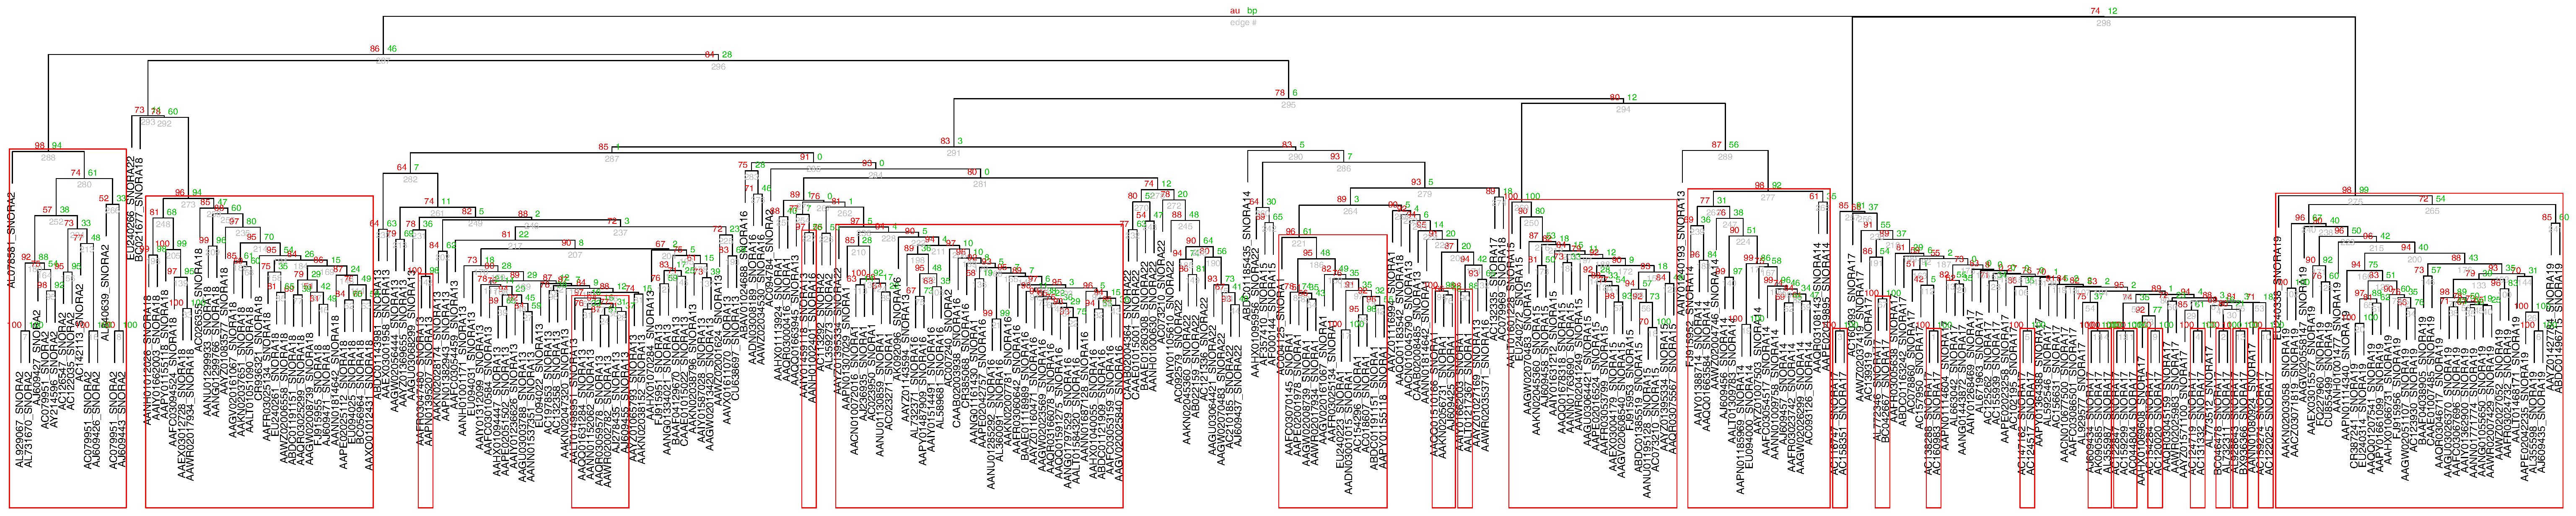
\epsfig{file = snornal140_dotaligner_g4_bootstrap1000.eps, width = 1\textwidth}}
  \caption{\GRAY{Automated hierarchical clustering of 300 sequences from 10 H/ACA
  snoRNA families. The dissimilarity matrix was calculated through \dotaligner{}
  with gap penalty 4. The clustering was conducted by the R-package \pvclust{}
  with multiscale bootstrap resampling with number of bootstrap 1000. We define
  clusters (red rectangles) as Approximately Unbiased (AU) \textit{p}-values $>$
  0.95 rejecting the hypothesis that ``the cluster does not exist`` with
  significance level 0.05.}}
  \label{fig:dotaligner_g4_cluster}
\end{figure*}


\subsection{Fragmented RFAM sequences} 

Local alignment, simulating genomic screens. More emphasis on qualitative clustering


\subsection{ A unified RNA structure clustering pipeline }

\noindent We implemented a user-friendly pipeline that automates all steps required 
for the detection of homologous RNA secondary structure motifs from a set of user-
provided sequences. The pipeline is implemented in BASH programming language and is 
designed for execution on a high performance computing server (currently, only SGE 
is supported). This enables non-specialists to complete such an analysis with 
minimal bioinformatics knowledge, while facilitating parameter modification and 
customization for advanced users. 

In summary, the pipeline performs the following tasks on a fasta file input:
\begin{enumerate}
\item Generates base-pairing probability matrices for each sequence with RNAfold's parition function algorithm 
\item Performs all-vs-all pairwise alignment in parallel with DotAligner (and/or CARNA, locarna, ....)
\item Generate (dis)similarity matrix from pairwise alignment scores 
\item Perform hierarchical clustering and bootstrap significance testing with \pvclust{} (Suzuki R and Shimodaira H. Bioinformatics 2006).
\item Extract the sequences and associated guide trees for significant clusters
\item Render a consensus secondary structure motif using the multiple structure alignment tool mlocarna
\end{enumerate}


\subsubsection{ On consensus hierarchical clustering }

We are investigating the practicality and efficiency of a consensus
hierarchical clustering approach, where the (dis)similarity matrices of
different pairwise structure alignment algorithms are concurrently employed for
cluster analysis. \textbf{This is cutting-edge stuff and Luis will report back
soon. }


\subsubsection{ On multiple structure alignment and 2D motif rendering }

Generating a multiple structural alignment at the end of the pipeline is an
important but tricky step.  Right now, we are using mlocarna for this, which to
my knowledge is the only tool that can produce such output without too much
fuss. However, there is a substantial concern that arises from its use:
\dotaligner and mlocarna use fundamentally different alignment algorithms. This
caveat is somewhat resolved by enforcing mlocarna to use the guide tree
produced from the all-vs-all (dis)similarity matrix from \dotaligner . Mlocarna
will still align the sequences based on their consensus structure, therefore
some additional benchmarking may be required. N.B., we can dictate which
pairwise aligner (or probabilistic aligner) to be used by mlocarna its
execution parameters, although mlocarna may ignore this when a guide-tree is
provided---thus employing locarna to produce intermediate alignments even when
only 2 sequences are involved. \textbf{CHECK THIS WITH SEBASTIAN WILL }

Some more specific points to consider: 
\begin{itemize}
\item --threads=X seemingly doesn't affect mlocarna performance. Is this only implemented for pairwise comparisons? 
Generating the intermediary alignments uses one CPU. Perhaps --cpu=X will work? 
\item RNAPLfold is used for longer input sequences, right? Is this because it overcomes sequence length discrepancies? 
Should we enfore a size limit on the input sequences (either trim or extend the input to XX nucleotides divergence)?
\item Try option \texttt{--pw-aligner path/to/DotAligner} and see if it will give more reliable consensus structure
\item Test whether the speed limitation of iterative refinement (\texttt{ --iterations=XX}) will be compensated by 
better quality alignments
\item Will this cause (m)locarna to use the entire dot plots for the alignment? Test the effect of the following 
parameters \texttt{--probabilistic --consistency-transformation --it-reliable-structure=XX}. 
\end{itemize} 
% --plfold-span=${SPAN} --plfold-winsize=${WINSIZE} \
% --probabilistic --consistency-transformation 
% --it-reliable-structure=10 


\section{\uppercase{Discussion}}

\noindent The application of \dotaligner{} is a fastly
calculated similarity score between two probability matrices to enable their
subsequent clustering.  Similar to \carna{}, which also does not garanty the
optimal solution, \dotaligner{} is not deterministic.

We plan to integrate the proposed method in a pipeline that screens regions of
interest for structured RNA domains in a collection of RNA molecules.  The so
far presented approach finds only global alignments. This strategy is
applicable for input sequences of similar lengths or if one sequence is
considerably shorter (due to the usage of free end gaps). However, local
alignment is favorable if both input sequences are long. Despite of the
partition function version of the local alignment problem is available, its
application dramatically increases the search space and, thus, the running
time. \RED{As alternative, a possible screening pipeline may comprise window
based thermodynamic folding, \eg{} by \rnaplfold{}
\cite{Bernhart:Hofacker:Stadler:Local_RNA_base:2006}, and filter regions of
high intra-molecular binding probabilities in a pre-processing step, \eg{} by
using \rnalocal{} \cite{Dotu19908358}, followed by the presented alignment tool
\dotaligner. SHOULD WE INCLUDE THIS ANALYSIS IN THIS PAPER AND IF YES WHERE?}
The pre-selection of local structural potential may improve the boundaries of
common structured RNA domain. 

\dotaligner{} can also be extended for multiple alignments, similar to the strategy
implemented in \pmmulti{} \cite{Hofacker15073017}, and the generation of
phylogenetic trees. This may replace or support the hierarchical clustering
approach used here. In addition, both may serve as input for RNA secondary
structure predictors, such as \petfold{} \cite{Seemann2008} unifying
thermodynamic and evolutionary information. 


\section*{\uppercase{Acknowledgements}}

\noindent I thank the Carlsberg foundation for my travel grant. Sk\aa l! \\
MAS is funded in part by a Cancer Council NSW project grant and 



\vfill
\bibliographystyle{apalike}
{\small
\bibliography{dotaligner}}


\vfill
\end{document}

